\subsection{From an Attempt to a Learner Record}
\label{sec:learner-state}
The observation pipeline separates identifying a concept from assessing an
answer. A turn can mention several concepts, but the primary-concept rule assigns
its assessment only to one unambiguous target; tied or weak attribution remains
unassessed. A mention therefore need not count as a correct or incorrect attempt.
The committed observation retains its concept identifiers, assessment outcome,
source references and course/release scope.

Figure~\ref{fig:learner-state} distinguishes the two consumers of stored activity.
Completion uses assessed student evidence; the default planner uses the much
simpler job-snapshot proxy. Their fields are not interchangeable.

\begin{figure}[htbp]
\centering
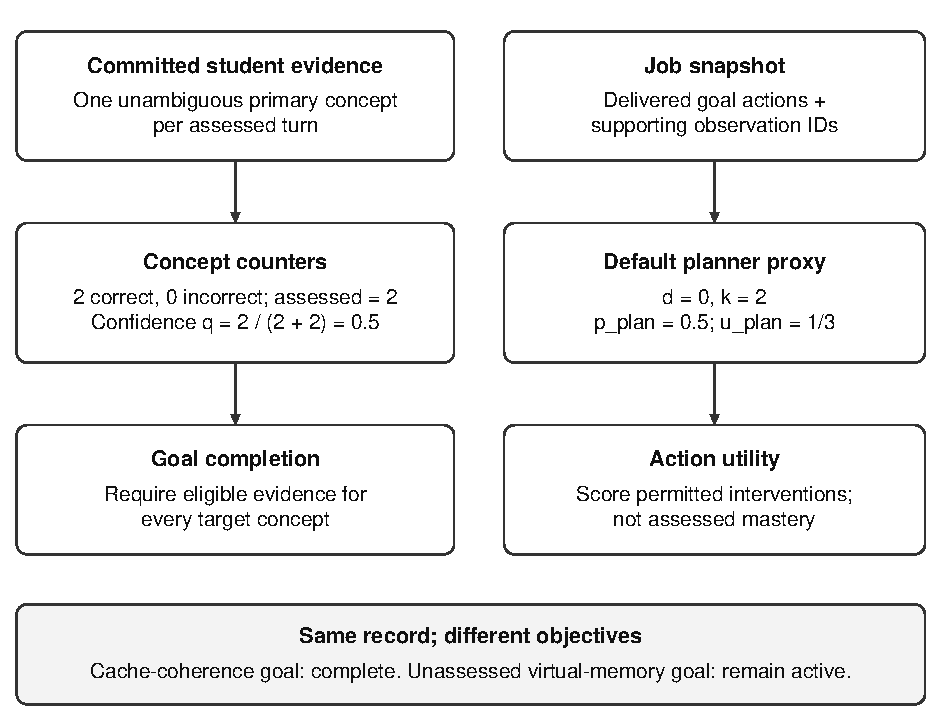
\includegraphics[width=\linewidth]{../../../reports/figures/course-twin-learner-state.pdf}
\caption{Assessment evidence and the default planner proxy have separate consumers.}
\label{fig:learner-state}
\end{figure}
For concept $c$, the evidence-count implementation records total observations,
assessed observations $a_c$, and correct, partial and incorrect counts
$(n_c^+,n_c^\sim,n_c^-)$. On an eligible assessed observation, only the relevant
outcome counter increases. Its confidence field is
\begin{equation}
q_c=\min\!\left(0.95,\frac{a_c}{a_c+2}\right).
\label{eq:evidence-confidence}
\end{equation}
Two assessed attempts give $q_c=0.5$ regardless of whether they were correct.
Thus this field represents accumulated assessment evidence, not the probability
that the student has mastered the concept. A new revision and its delta are
saved together with the accepted turn; rejected or stale observations cannot
be used as committed evidence.

The current goal correction maps each active goal $g$ to exactly one objective
in the same published domain. Let $C(g)$ be that objective's nonempty concept set,
and $S_g$ indicate that the mapping and committed learner state have valid scope.
For the evidence-count learner state, completion is
\begin{equation}
\operatorname{complete}(g)=S_g\ \land\
\bigwedge_{c\in C(g)}
\left[n_c^+\geq2\ \land\ n_c^-=0\ \land\ q_c\geq0.5\right].
\label{eq:goal-completion}
\end{equation}
Missing or ambiguous mappings remain incomplete. For example, two correct
cache-coherence assessments can satisfy a cache-coherence objective but cannot
complete an unassessed virtual-memory objective. This is the boundary reproduced
in the service audit and tested after the correction (Section~\ref{sec:goal-study}).
The rule retains a limitation: an earlier incorrect count continues to block
completion in that state. It also does not parse a professor's free-text success
condition. A completed software goal is consequently a threshold decision,
not independently demonstrated mastery.

\FloatBarrier
\subsection{How the Planner Chooses a Teaching Action}
\label{sec:planning}
The event determines candidate actions and their fallback order. Repeated
confusion permits a hint/example followed by a diagnostic question; a misconception
reverses that order. An incomplete objective or inactivity permits an in-app
check-in, and due review permits retrieval practice. The application intersects
this set with the instructor's permitted actions and adds \emph{no action}.
Let the resulting set be $A$, and $a_0$ its first permitted action.

The guarded planner scores every $a\in A$ using an inspectable forward model:
\begin{equation}
U(a)=\operatorname{clip}_{[-2,2]}
\left(G(a)+0.45O(a)+F(a)+B(a)-0.9R(a)-I(a)\right).
\label{eq:planning-utility}
\end{equation}
$G$ is a heuristic immediate-gain term weighted by estimated need and spacing;
$O$ rewards obtaining another observation when uncertainty is high; $F$ adds a
bounded look-ahead term; $B$ favours a hint or diagnostic question for repeated
errors; $R$ penalizes evidence risk and repetitive check-ins; $I$ is the
action-specific interruption cost. These constants are hand-specified, not
learned causal effects. Appendix~\ref{sec:planner-math} gives the exact terms.

Let $a^*=\arg\max_{a\in A}U(a)$, breaking ties by event order, and $a_L$
be the model proposal. Table~\ref{tab:planner-rules} makes the choice explicit;
Figure~\ref{fig:planner-decision} then applies it to the worked example.
Authorization and content validation remain separate from action selection.

\begin{table}[htbp]
\centering\small
\caption{Guarded-planner decision rules.}
\label{tab:planner-rules}
\begin{tabularx}{\linewidth}{@{}Yccccc@{}}
\toprule Condition / outcome & \shortstack{No\\evidence} & \shortstack{Invalid\\proposal} & \shortstack{Not\\best} & \shortstack{Small\\gain} & Adopt \\ \midrule
Authorized evidence ready? & N & Y & Y & Y & Y \\
Proposal valid; every step permitted? & -- & N & Y & Y & Y \\
Proposal selects analytic best ($a_L=a^*$)? & -- & -- & N & Y & Y \\
Improves fallback by at least 0.04? & -- & -- & -- & N & Y \\\midrule
Selected action & None & $a_0$ & $a_0$ & $a_0$ & $a_L$ \\
\bottomrule
\end{tabularx}
\end{table}

Ordinary provider/proposal failures retain the fallback; provider-identity errors propagate
to the failure boundary. If the model proposes the fallback itself, the action
is unchanged even though model-supplied metadata may be retained.

\textbf{What state actually reaches this planner.}
The planner receives a structured state summary, called a planning-state card.
The default adapter does not connect the detailed counts above to a calibrated
estimator. With $d$ delivered goal actions and $k$ supporting observation
identifiers, it supplies
\begin{equation}
p_{\rm plan}=\min\!\left(0.95,\frac{d+1}{d+2}\right),
\qquad u_{\rm plan}=\frac{1}{k+1}.
\label{eq:planner-proxy}
\end{equation}
The field named mastery probability therefore rises from $0.5$ to $2/3$ after
one delivery even without a student answer. Its uncertainty input counts
identifiers, not necessarily assessed attempts. Repeated-error state is derived
from the event category, and elapsed-observation time is not populated by this
adapter. These are planning proxies, distinct from Equation~\ref{eq:evidence-confidence}
and the simulator's hidden mastery. The BKT/PFA comparisons in
Section~\ref{sec:timing-comparison} are experimental alternatives, not evidence
that those estimators already drive the retained application.

\textbf{A worked calculation.}
For a repeated-confusion event with both actions permitted, zero delivered goal
actions, two supporting identifiers and ready evidence, the default adapter gives
$p_{\rm plan}=0.5$, $u_{\rm plan}=1/3$ and zero goal progress. At look-ahead
depth two, the code yields $U(\text{hint})=0.325$ and
$U(\text{diagnostic question})\approx0.267$. The event fallback is already the
hint, so a model-proposed question cannot replace it. This calculation explains
the implemented rule; it is not a recorded model response or evidence that a
hint is educationally optimal.

\begin{figure}[htbp]
\centering
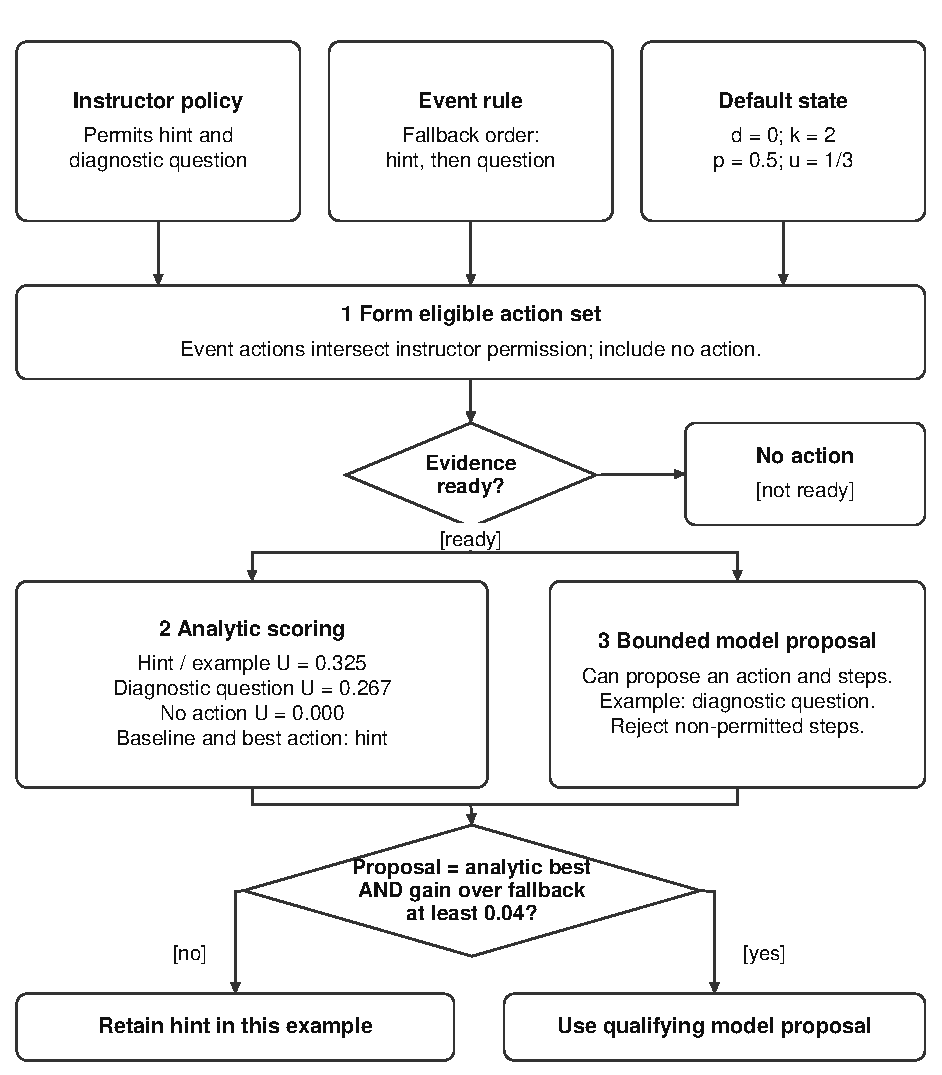
\includegraphics[width=\linewidth]{../../../reports/figures/course-twin-planner-decision.pdf}
\caption{Repeated-confusion example: the proposed diagnostic question cannot replace the higher-scoring hint.}
\label{fig:planner-decision}
\end{figure}
